\chapter{Sólo un poco más de Astronomía}

\lettrine[lines=2]{C}{ecilia y Antonia} se alejaban del Observatorio
con paso tranquilo y ligeramente melancólico, recorriendo una vez más
los interminables pasillos de Harvard. El Sol las acariciaba
cálidamente a medida que pasaban frente a los amplios ventanales que
iluminaban los claustros. El silencio que las acompañaba era
suficientemente elocuente, y las dos se dejaron arropar por él, por su
amistad y por la luz solar.

De pronto Cecilia detuvo sus pasos:

---¿Escuchaste algo?  ---pre\-gun\-tó.

Antonia se detuvo a su vez y prestó atención; tras unos breves
instantes respondió:

---No, nada... ¿Por?

Cecilia sacudió la cabeza levemente; con una sonrisa retomó la marcha:

---Por nada; me pareció sentir que nos llamaban.

No dieron más que unos cuantos pasos cuando ahora fue Antonia quien se
detuvo. Se encontraban en ese momento al lado de uno de los
ventanales. Giró sobre sí misma para enfrentarse a él. Tenía los ojos
cerrados; pareció disfrutar de la caricia del Sol sobre sus párpados
mientras respiraba profundamente. Cecilia la contemplaba con ternura:
no recordaba haber visto antes a su amiga disfrutar de las sensaciones
delicadas y elementales que nos regala la naturaleza.

Antonia abrió los ojos y exhaló un fuerte suspiro. De las
profundidades del morral que siempre la acompañaba extrajo el reloj de
Sol digital que había impreso antes del comienzo de esta aventura.
Cecilia lo reconoció inmediatamente: era el mismo que vio en su
oficina en el capítulo \ref{cap:antonia}, y con cuyos rayos la asombró
en el capítulo primero.

---Me gustaría que discutiéramos algo ---propuso Antonia.

\section{Un \emph{bug} más bien astronómico}


---En el capítulo \ref{cap:poquito-de-astronomia} concluimos que el
cuerpo del reloj debe colocarse de forma paralela al eje de la Tierra
---e\-vo\-có Antonia---; en otras palabras, inclinado un ángulo igual a
nuestra latitud y dispuesto en el plano vertical que une los puntos
cardinales Norte y Sur.

\begin{figure}[ht]
  \centering
  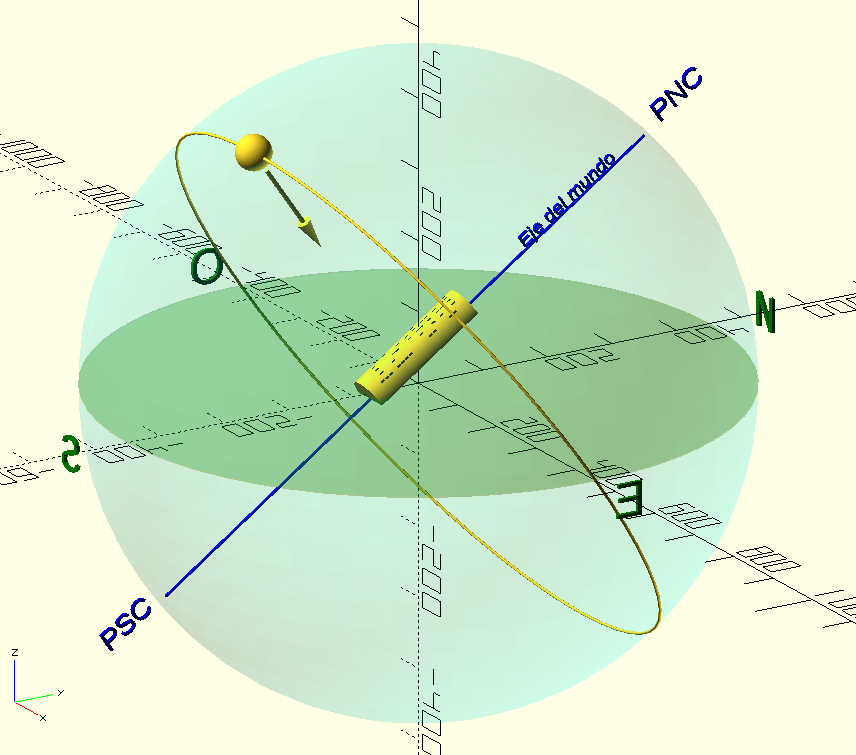
\includegraphics[width=.6\textwidth]{imagenes/orientacion-reloj.png}
  \caption{Antonia y Cecilia concluyeron en el capítulo
    \ref{cap:poquito-de-astronomia} que el reloj debe orientarse
    paralelamente al eje terrestre.}
  \label{fig:orientacion-reloj-apendice}
\end{figure}

Cecilia lo recordaba perfectamente.

---La latitud de Harvard es de unos 35º Sur\footnote{Ya entendí
  todo. (Nota del Editor)} ---con\-ti\-nuó su amiga---; puse una
marquita en el soporte para poder inclinar el cuerpo del reloj con
certeza.

Con movimientos pausados, casi ceremoniosos, Antonia se inclinó hacia
el piso para ubicar el reloj de Sol digital orientado de la manera en
que habían deducido que debía colocarse. Sin embargo, para sorpresa de
Cecilia ningún dígito se formó debajo del mismo; miró a su amiga sin
poder disimular un gesto de alarma:

---¿Qué pasó? ---preguntó, visiblemente consternada ante la 
figura \ref{fig:reloj-solsticio-mal}.

\begin{figure}[ht]
  \centering
  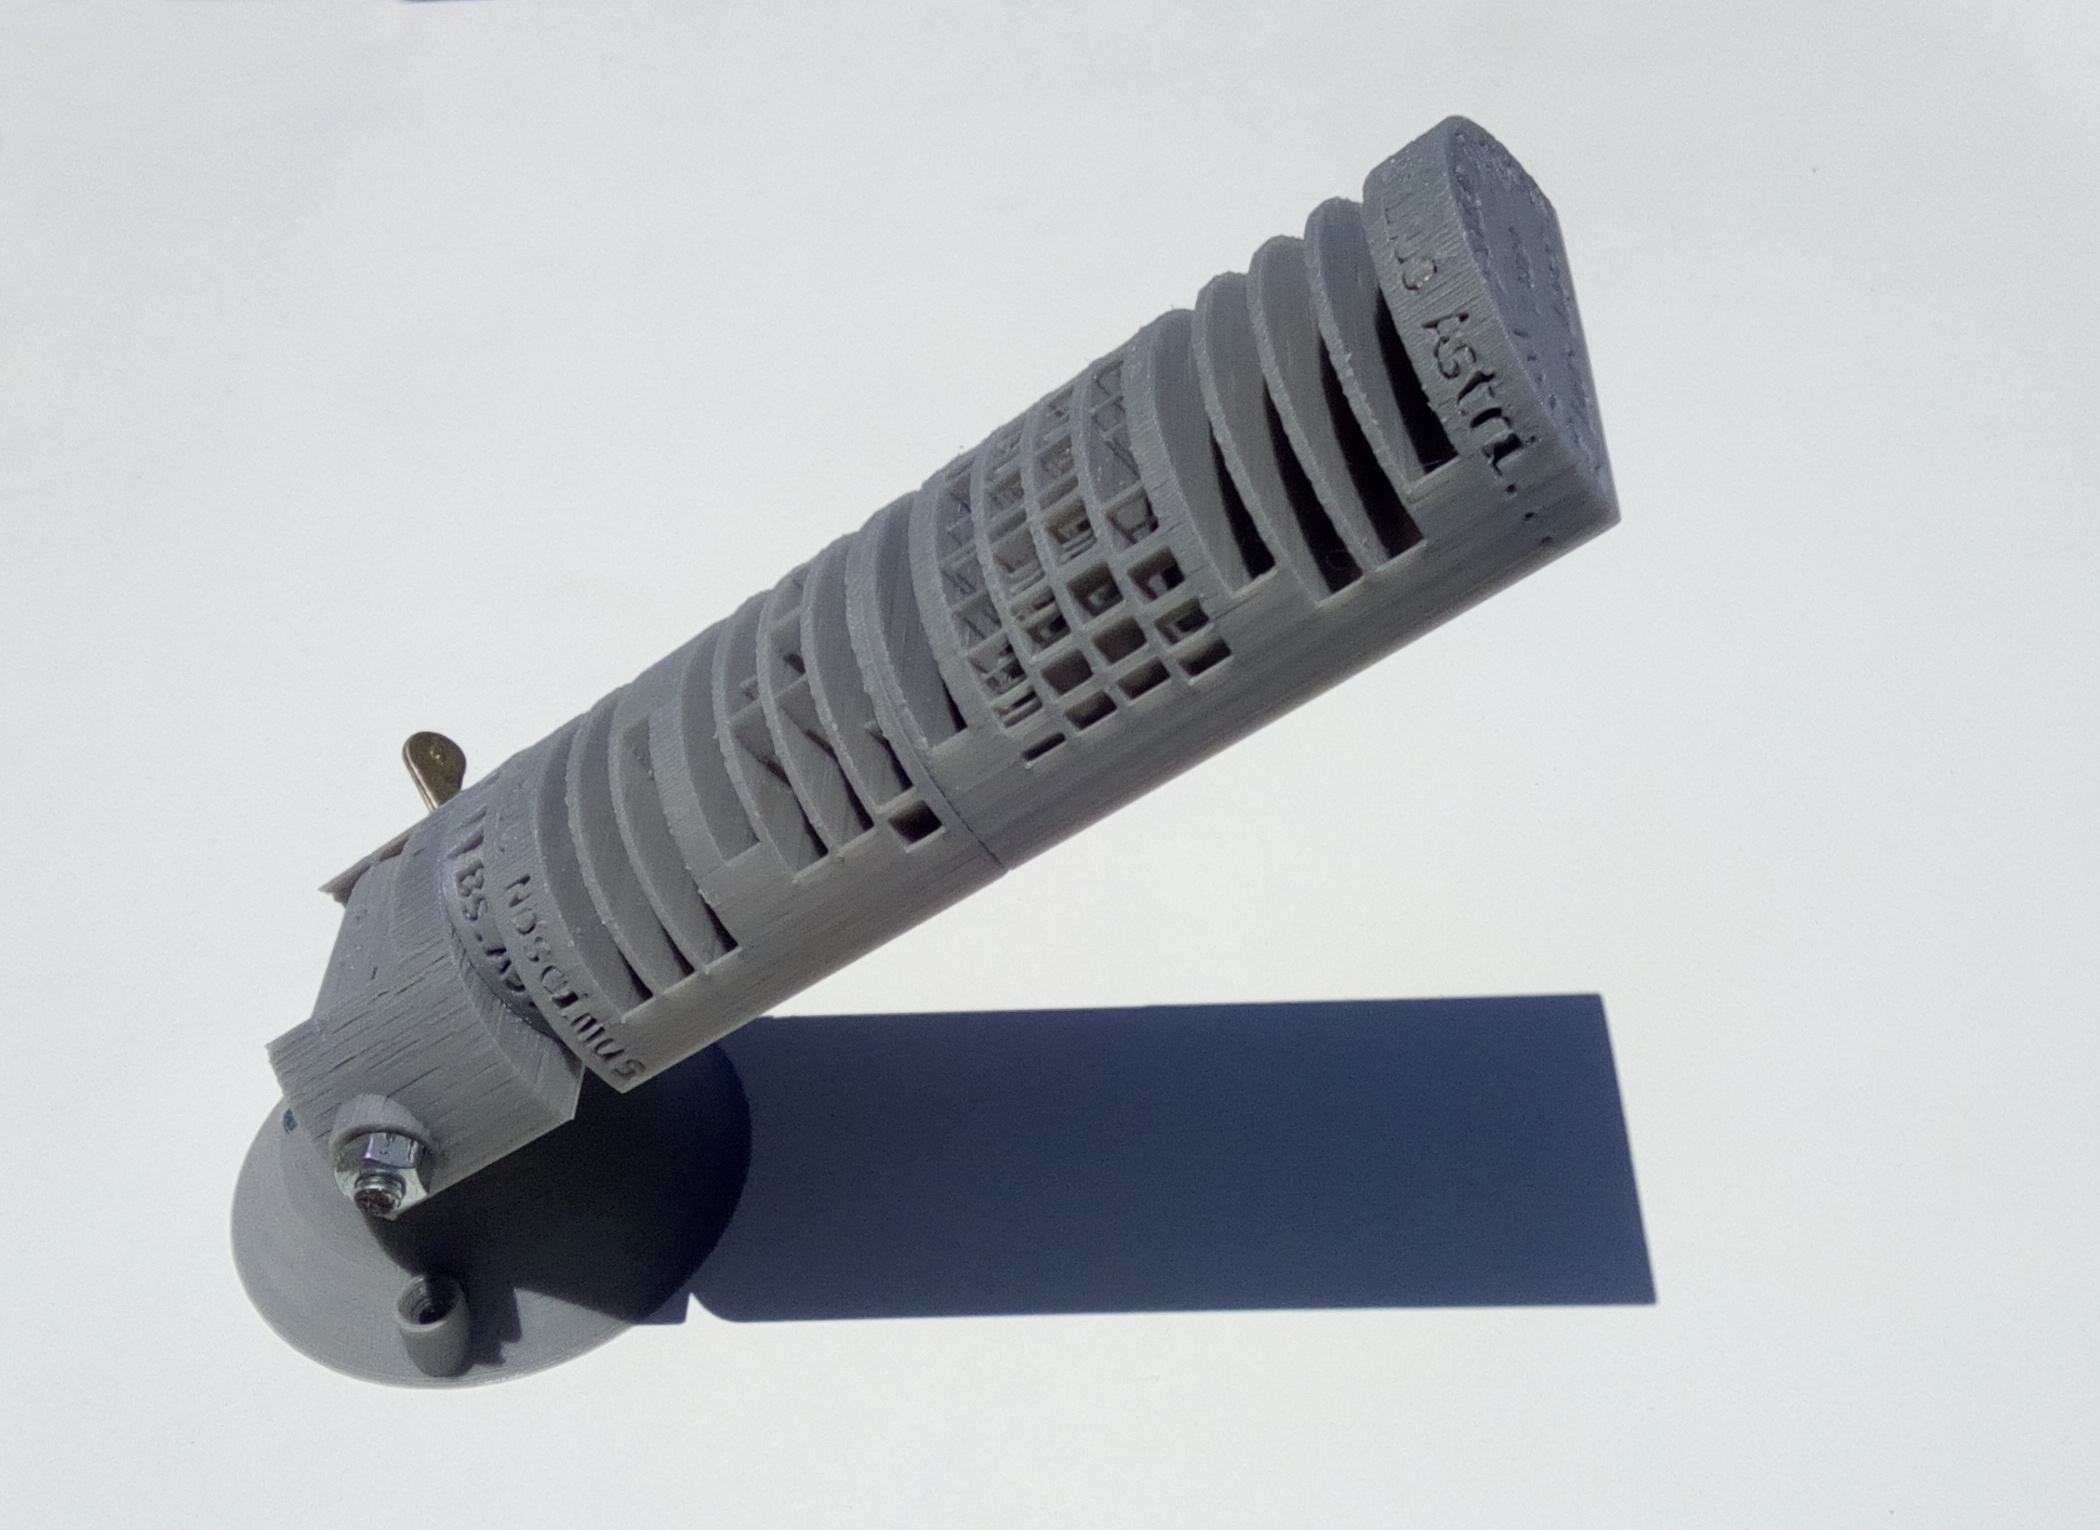
\includegraphics[width=.65\textwidth]{imagenes/reloj-solsticio-mal}
  \caption{El reloj de Sol, para alarma y angustia de Cecilia, no
    indica la hora.}%\iftoggle{libro}{\vspace{128in}}{}
  \label{fig:reloj-solsticio-mal}
\end{figure}

---Tranquila ---contestó Antonia con una sonrisa---. Se trata de un
pequeño detalle que yo tampoco tuve en cuenta la primera vez que probé
el reloj frente al Sol, y sobre el que no quise llamar tu atención en
el capítulo \ref{cap:poquito-de-astronomia}... ¡Demasiados problemas
teníamos por delante, y de índole más urgente y teórica, antes que
éste, de naturaleza apenas `práctica' y de muy fácil solución..!

La alarma de Cecilia fue reemplazada por una suerte de indignada
sorpresa: ¿El hecho de que el reloj no mostrase la hora le parecía a
Antonia un detalle menor y de índole meramente ``práctica''? Cecilia
conocía ya de sobra la inclinación de su amiga por las ideas ``puras''
y la teoría; inclinación ésta que a veces la llevaba a mirar con
desdén todo aquello que supusiera una aplicación o resultado concreto
y material. Pero esto ya le parecía el colmo.

Antonia, indiferente a la sorpresa de su amiga, continuó disertando:

---El problema se manifiesta cuando el Sol se encuentra relativamente
alejado del Ecuador Celeste ---explicó---. En ese caso, los rayos
solares no pueden pasar por los huecos que se encuentran óptimamente
dispuestos sólo cuando el Sol se encuentra en dicho plano: en otras
palabras, más bien cerca de la primavera o el otoño.

\begin{figure}[ht]
  \centering
  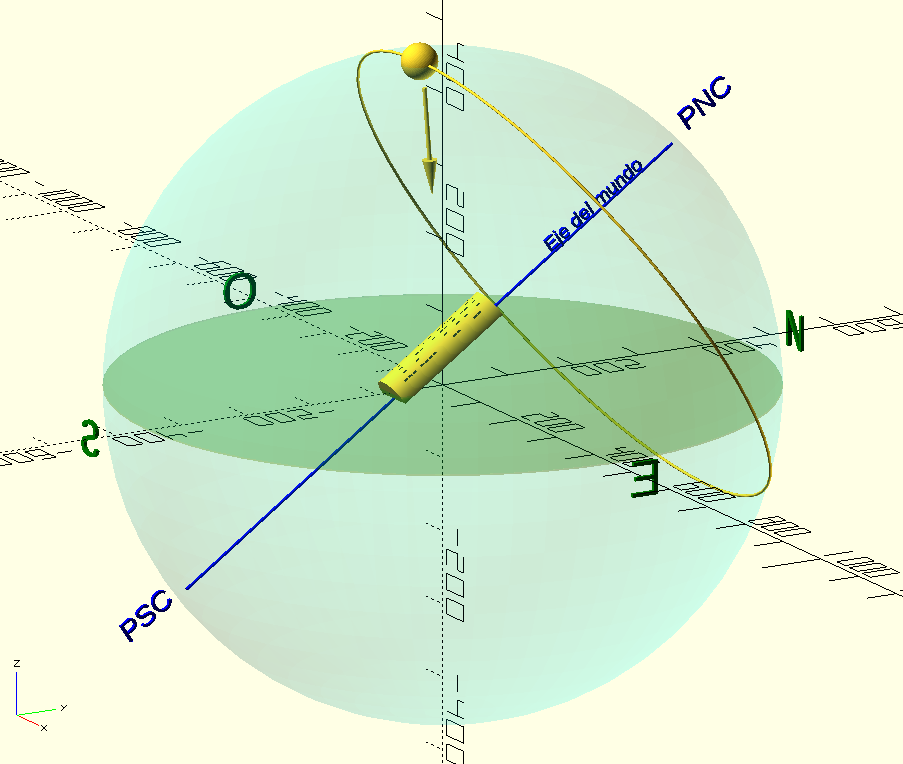
\includegraphics[width=.49\textwidth]{imagenes/orientacion-reloj-solsticio.png}\hfill
  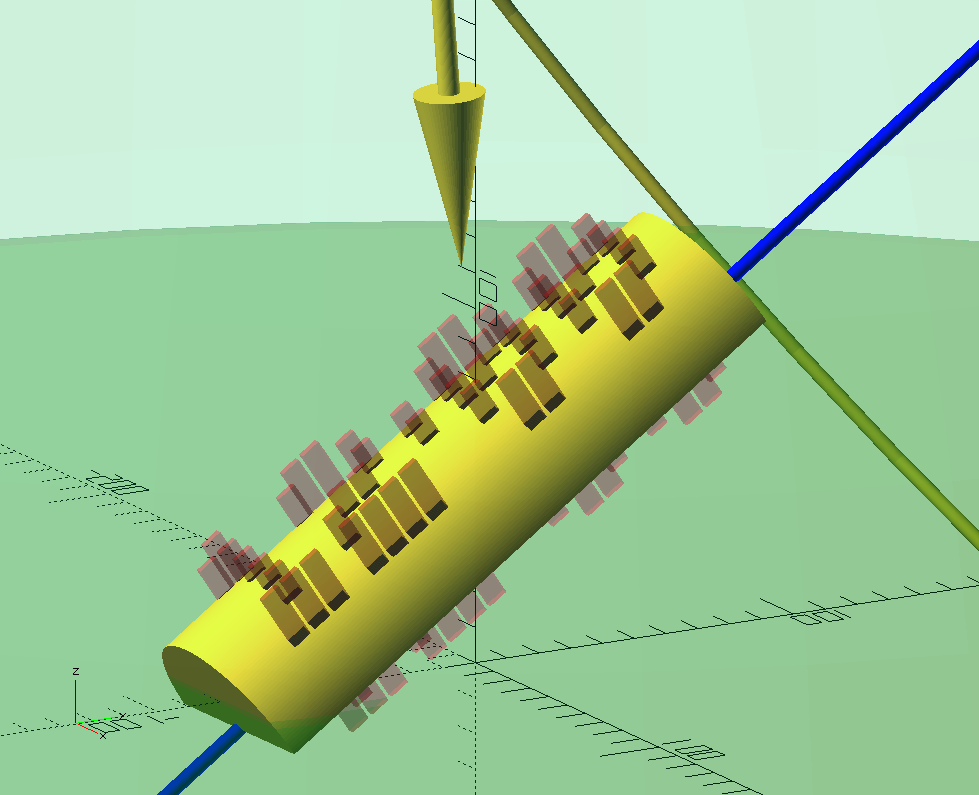
\includegraphics[width=.49\textwidth]{imagenes/orientacion-reloj-solsticio-zoom.png}
  \caption{Cuando el Sol se encuentra muy alejado del Ecuador Celeste
    (o sea, cerca del invierno o del verano), sus rayos no alcanzan a
    atravesar los agujeros del reloj, que fueron dispuestos para
    recibirlos de manera perpendicular a su cuerpo.}
  \label{fig:orientacion-reloj-2}
\end{figure}

Cecilia pudo apreciar con claridad el problema en la figura
\ref{fig:orientacion-reloj-2}. Imaginó una forma de resolverlo y, aunque
en el fondo no le gustaba, se sintió obligada a proponerla:

---¿Aumentamos el ancho de los pixeles? De esta manera los rayos
solares podrán atravesar los agujeros, al menos de soslayo, aun en los
solsticios.

Antonia frunció el gesto; a ella tampoco parecía gustarle esa
solución.

---Lo que proponés no es, por supuesto, ineficaz ---co\-men\-tó---. El
inconveniente es que eso nos obligaría a alargar mucho los
pixeles... Te confieso que no hice las cuentas, pero estoy segura de
que resultaría un reloj de Sol demasiado largo. Tal vez ni siquiera
podríamos imprimirlo.

Cecilia pensó que siempre podían imprimir el reloj por partes y luego
pegarlas; pero prefirió dejar que Antonia se tomara su tiempo para
ofrecer la solución que, sin duda, consideraría óptima.

---Además, si alargamos los pixeles obtendremos sobre el piso horas
muy anchas en los equinoccios y más angostas en los solsticios
---a\-ña\-dió Antonia, como si necesitara refutar del todo la
propuesta de Cecilia antes de adelantar la suya propia. Cecilia pensó
que ésta quizá no sería tan buena, después de todo, si antes era
preciso destacar tantos defectos en la otra.

Antonia hizo un breve silencio mientras miraba el reloj de Sol digital
con gesto reconcentrado; parecía buscar la mejor manera de presentar
su solución. 

---Mirá, para mí, lo mejor es simplemente modificar, los días que
resulte necesario, el ángulo de inclinación del reloj para que los
agujeros resulten paralelos a la dirección de los rayos solares
---propuso finalmente y con el aire de seguridad y suficiencia con el
que soltaba las ideas que, en el fondo, sentía que no podía justificar
del todo: otro más de sus defectos docentes.

\begin{figure}[ht]
  \centering
  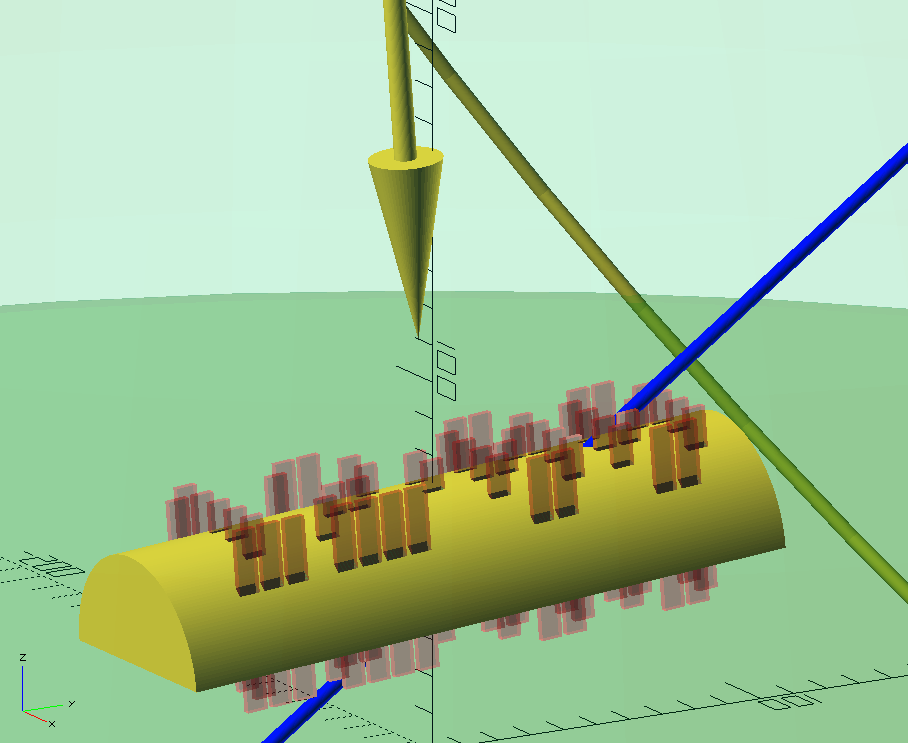
\includegraphics[width=.5\textwidth]{imagenes/reorientacion-reloj-solsticio-zoom.png}
  \caption{Antonia propone modificar la inclinación del reloj para que
    su cuerpo resulte, cada día, perpendicular a los rayos solares.}
  \label{fig:reorientacion-reloj}
\end{figure}

\begin{figure}[ht]
  \centering
  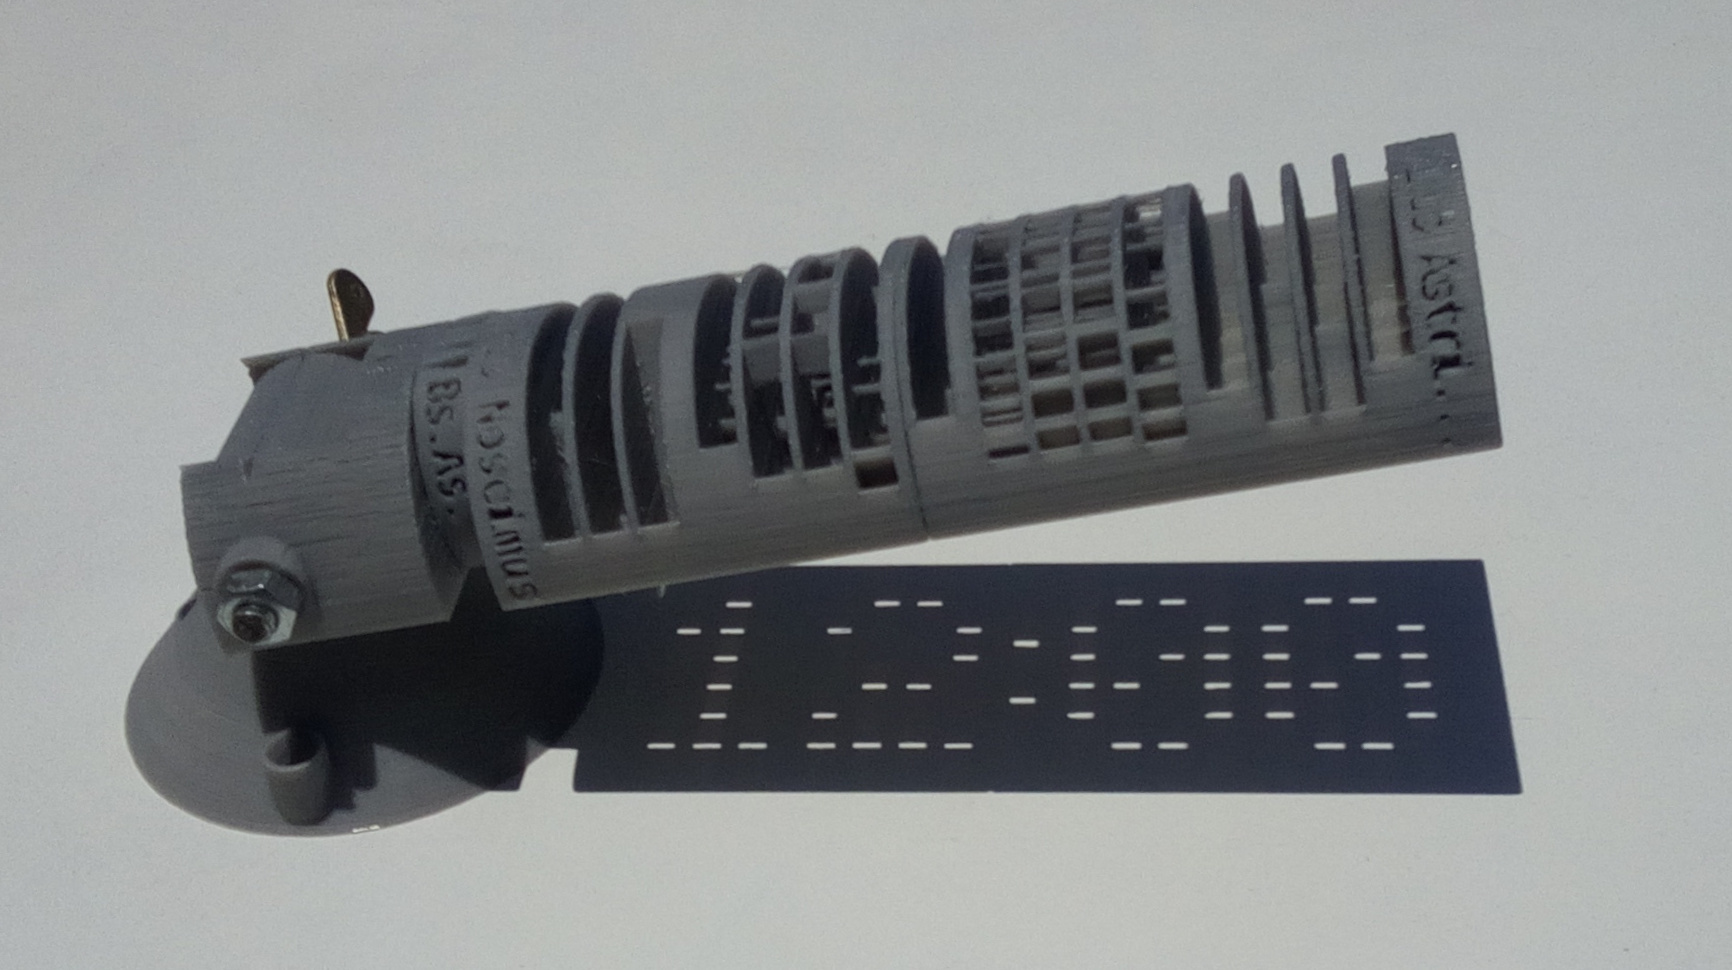
\includegraphics[width=.7\textwidth]{imagenes/reloj-solsticio-bien}
  \caption{El reloj de Sol, debidamente inclinado, indica la
    hora aun en los solsticios.}%\iftoggle{libro}{\vspace{128in}}{}
  \label{fig:reloj-solsticio-bien}
\end{figure}

Cecilia se cruzó bruscamente de brazos: se sentía francamente
decepcionada.

---¿Modificar la inclinación del reloj? ---repitió en forma de
pregunta, sin disimular un tono de frustración.

---Sí ---replicó Antonia, alzando cejas y hombros como si hubiera
propuesto la solución más natural del mundo.

Cecilia mantenía los brazos cruzados, y ahora tamborileaba con la
punta del pie contra el piso. Podía ver que la solución funcionaba,
pero le resultaba un tanto chapucera. Tanto ella como Antonia
mantenían los ojos fijos en el reloj, que silencioso e indiferente
mostraba la hora con puntualidad solar.\footnote{¿Y? ¿Ya está?  ¿Pero
  ahora qué hacemos? (Nota del Editor)}$^,$\footnote{Nosotros, nada:
  si después de \pageref{sec:final_apendice} páginas no fuimos capaces
  de permitir a nuestro querido e improbable lector que encuentre sus
  propias respuestas por sí mismo, triste librito sería éste. (Nota de
  Antonia, Cecilia y Luis)}\label{sec:final_apendice}






%%% Local Variables:
%%% mode: latex
%%% TeX-master: "../libro"
%%% End:
